\section{Benchmarking}
\label{sec:benchmarking}


We present a set of experiments to evaluate the efficacy of the proposed modular code generation tool (\ourTool) with \simulink. 
In the first experiment, we select benchmarks that span across different application domains such as medical, physics, and industrial automation, to illustrate the \emph{diversity} of the proposed approach.
We then compare each of these benchmarks against \simulink in terms of execution time and maximum memory usage.
In the second experiment, we evaluate the \emph{scalability} of \ourTool and \simulink as the number of cells in the \ac{NHC} model increases. 


\subsection{Experimental set-up}
\label{sec:experimentalSetUp}
The following steps were considered in order to achieve a fair comparison between \ourTool and \simulink:

\begin{description}[\IEEEsetlabelwidth{Step Size}\IEEEusemathlabelsep]
	\item[\textbf{Solver}] To reflect the synchronous execution model, we used a discrete solver with a fixed step in \simulink, namely \texttt{ode1} (Forward Euler).
	
	\item[\textbf{Step Size}] For all benchmarks the step size in \simulink is fixed to $0.01$ milliseconds.
	The same step size is also used in \ourTool, $\delta = 0.01$ milliseconds.
	
	\item[\textbf{Time}] All benchmarks were simulated for $10$ seconds of simulation time.
	Based on a step size of $0.01$ milliseconds this translates to $1$ million ticks in \ourTool.
\end{description}

The experiments were evaluated using an Intel~i7-4790 processor with 8~GB RAM on Windows~7. 


\subsection{Diversity}

\begin{figure}[htbp]
	\centering
	\subfigure[Execution time (ms) \label{fig:executionTime}]{
		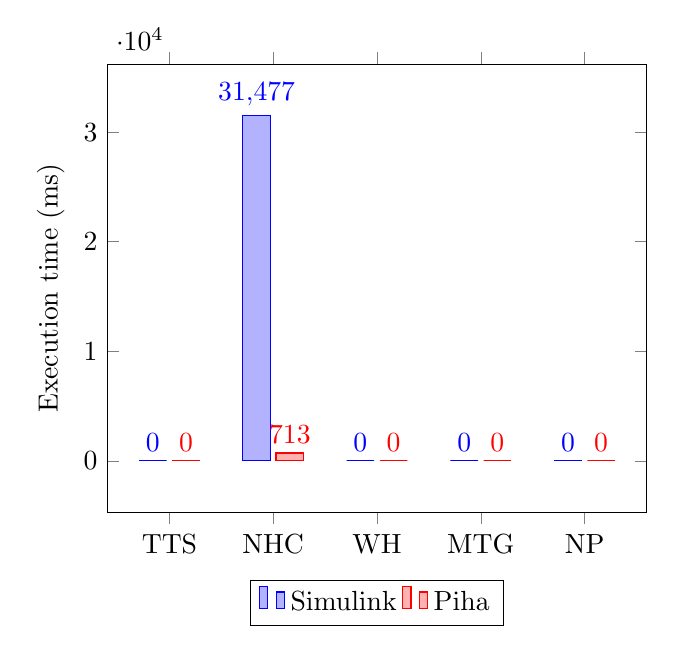
\begin{tikzpicture}
\begin{axis}[
	ybar,
	enlargelimits=0.15,
	legend style={
		at={(0.5,-0.15)},
		anchor=north,
		legend columns=-1
	},
	ylabel={Execution time (ms)},
	symbolic x coords={TTS, NHC, WH, MTG, NP},
	xtick=data,
	nodes near coords,
	nodes near coords align={vertical},
]

%Simulink
\addplot coordinates {
	(TTS,0)
	(NHC,31477)
	(WH,0)
	(MTG,0)
	(NP,0)
};

%Piha
\addplot coordinates {
	(TTS,0)
	(NHC,713)
	(WH,0)
	(MTG,0)
	(NP,0)
};

\legend{Simulink, Piha}

\end{axis}
\end{tikzpicture}

	}
	\subfigure[Memory requirement (MB) \label{fig:memoryRequirement}]{
		\begin{tikzpicture}
\begin{axis}[
	ybar,
	enlargelimits=0.15,
	legend style={
		at={(0.5,-0.15)},
		anchor=north,
		legend columns=-1
	},
	ylabel={Memory Requirement (MB)},
	symbolic x coords={TTS, NHC, WH, MTG, NP},
	xtick=data,
	nodes near coords,
	nodes near coords align={vertical},
]

%Simulink
\addplot coordinates {
	(TSN,0)
	(NHC,200)
	(WH,0)
	(MTG,0)
	(NP,0)
};

%Piha
\addplot coordinates {
	(TSN,0)
	(NHC,1.3)
	(WH,0)
	(MTG,0)
	(NP,0)
};

\legend{\simulink, \ourTool}

\end{axis}
\end{tikzpicture}

	}
	\caption{Comparison of the execution time (in ms) and memory requirement (in MB) between \simulink and \ourTool for the benchmarks in Table~\ref{tab:benchmarks}.}
	\label{fig:results}
\end{figure}

For the purposes of this experiment, we use the five benchmarks presented in Table~\ref{tab:benchmarks}.
The table also presents the number of locations (\#L) in each hybrid automata.
For example, $(2, 2, 2)$ denotes that the \acf{TTS} benchmark is described using three \acp{HA} each with two locations.
More details about the benchmarks and their implementation in \ourTool and \simulink are available online~\cite{githubBenchmarks}.

For all the benchmarks, the executable for the \simulink models are generated using the in-built Real-time Workshop\textsuperscript{\textregistered} C code generator.
Similarly, for \ourTool, we generate equivalent C code and compile to an executable using GCC.
The execution times and memory requirements of the generated executables are reported below and illustrated in Figure~\ref{fig:results}.

\textbf{Execution time:} 
Figure~\ref{fig:executionTime} shows that...

\textbf{Code size:}
Figure~\ref{fig:memoryRequirement} shows that...

On average, the code generated by \ourTool executes ?? times faster, while requiring ?? times less memory when compared to \simulink.

\begin{table*}
	\centering
	\caption{Benchmark descriptions
	\label{tab:benchmarks}}
\begin{tabular}{ | c | c | c | l | } \hline
\textbf{Benchmarks}
	& \textbf{Domain} 
	& \textbf{\#L } 
	& \textbf{Description} \\ \hline

	\acf{TTS}
		& Physics~\cite{Pedro2005}
		& $(2, 2, 2)$
		& Three thermostats heating a room to keep it warm\\ \hline
		
	\acf{NHC}
		& Biology~\cite{chen201487}
		& $(4^{33})$
		& Captures the electrical conduction system of a heart with $33$ nodes\\ \hline

	\acf{WH}
		& Physics~\cite{raskin05}
		& $(4, 4)$
		& Models the heating of water in a tank \\ \hline
		
	\acf{MTG}  
		& Industrial automation~\cite{Costello2013}
		& $(2, 3^{30})$
		& Models the behaviour of a gate and $30$ trains at a rail road crossing\\ \hline
		
	\acf{NP}
		& Industrial automation~\cite{alur2015book}
		& $(3^{30}, 3^{30})$
		& Switches between two fuel rods in 30 reactors to avoid nuclear meltdown\\ \hline
	
	
 \end{tabular}
 \end{table*}


\subsection{Scalability}

\begin{figure}[htbp]
	\centering
	\begin{tikzpicture}[yscale=0.85]
\begin{axis}
[
	xlabel={Number of Heart Nodes},
	ylabel={Execution Time ({s})},
	axis y line = left,
	axis x line = bottom,
	xmin=0000,
	xmax=1000,
	ymin=0,
	ymax=150,
	ytick={0, 10, 50, 100, 150},
	yticklabels={0, 10, 50, 100, 150},
	extra tick style={grid=major},
	legend style={
		at={(0.52,0.99)},
		anchor=north,
		legend columns=-1
	}
]

\addplot[color=blue!90,
	mark=square*,
	mark size=2
] table [
	x=n,
	y=s_t,
	col sep=comma
] {./figures/scalabilityGraphData.csv};
\addlegendentry{\simulink}

\addplot[color=red!90,
	mark=*,
	mark size=2
] table [
	x=n,
	y=p_t,
	col sep=comma
] {./figures/scalabilityGraphData.csv};
\addlegendentry{\ourTool}

\addplot[color=black!90,
	dashed,
	mark=.,
	mark size=2
] coordinates {
	(0,10)
	(1000,10)
} node[pos=0.8] (endofrealtime) {};
\node[above] at (endofrealtime) {Real Time};

\addplot[color=blue!90,
	dashed,
	mark=.,
	mark size=2
] coordinates {
	(297,126.448)
	(297,0)
};



\end{axis}
\end{tikzpicture}
	\caption{Scalability in  execution time of \simulink and \ourTool against number of cells}
	\label{fig:scalability}
\end{figure}

The purpose of the second experiment was to validate the scalability of \ourTool through the running example of the \ac{NHC} whilst comparing it to \simulink.
Code was generated for varying network sizes (33 cells, 66 cells, 99 cells, etc.) and the execution time recorded.
The experimental set-up was the same as described in Section~\ref{sec:experimentalSetUp}, ie. $1$ million ticks at a $0.01$ millisecond step size.

The most obvious feature of these results is that no data is recorded for \simulink for complexities greater than 297 cells. \simulink imposes an inbuilt requirement that the generated code use less than 2.1GB of memory and this discontinuity represents the point after which the memory requirement exceeds this limit\footnote{\simulink memory usage at 297 cells is 1.8GB}.

\begin{itemize}
	\item \ourTool has a smaller gradient
	\item \ourTool carries past this point that \simulink doesn't
	\item Point out the change in gradient around ~240 cells in \ourTool is due to cache size
	\item Mention the real time requirements for \ourTool vs \simulink
\end{itemize}